\documentclass[12pt]{article}
\usepackage[letterpaper, margin=1in]{geometry}
\usepackage{graphicx}
\graphicspath{{./Figures/}}
\usepackage{hyperref}
\usepackage{parskip}
\usepackage{amsmath}
\usepackage[framed, numbered]{matlab-prettifier}
\lstset{inputpath=../MATLAB}

\title{ELECENG 3TR4 Lab 1: Fourier Analysis}
\author{
    Aaron Pinto \\ pintoa9
    \and
    Raeed Hassan \\ hassam41
}

\begin{document}

\maketitle
\clearpage

% stuff goes here
\section*{Design Problem}
The output of a function generator is a square wave with 50\% duty cycle and the period of the wave is 0.1 ms. You may assume that the amplitude of the square wave is 1 Volt. Design a second order Butterworth filter so that any harmonics in the output is at least 23 dB below the fundamental sinusoid at 10 kHz, and the loss of the fundamental sinusoid due to filtering should be less than 2 dB. The purpose of this experiment is to generate a high amplitude sinusoidal signal out of a square wave (to have a high quality sinusoid, the amplitudes of harmonics should be sufficiently low). You should choose the cutoff frequency of the filter (i.e. 3 dB bandwidth of the filter) such that the above design constraints are met.


\section*{Determining the Frequency Response of the Filter}
% talk about getting the frequency response of the filter (frequencyResponse.m)
The first step we took was to implement a second order Butterworth filter in MATLAB and examine its frequency response. To simulate the filter, the transfer function of a second order Butterworth filter was used. The transfer function that was used for the second order Butterworth filter was provided in the textbook.
\begin{equation*}
    H(s) = \frac{1}{s^2 + 1.414s + 1}
\end{equation*}
% how the file works
The MATLAB script used to simulate the filter, frequencyResponse.m, generated the frequency response of the filter with its transfer function using the freqs function. A portion of the MATLAB code used to generate and plot the frequency response of the filter is shown below in Listing~\ref{listing:freq_response}.
% listing
\lstinputlisting[style=Matlab-editor, caption={Generating the Frequency Response of Second Order Butterworth Filter}, label={listing:freq_response}, firstline=23, firstnumber=23, lastline=53]{frequencyResponse.m}
% how we used the file
The MATLAB script was used to visualize the normalized frequency response of the filter, and to determine the attenuation provided by the filter at frequencies of interest (the fundamental frequency, and the frequency of the third harmonic). An example of plots generated by script is shown in Figure~\ref{fig:example_freq_response}.
\begin{figure}[h!]
    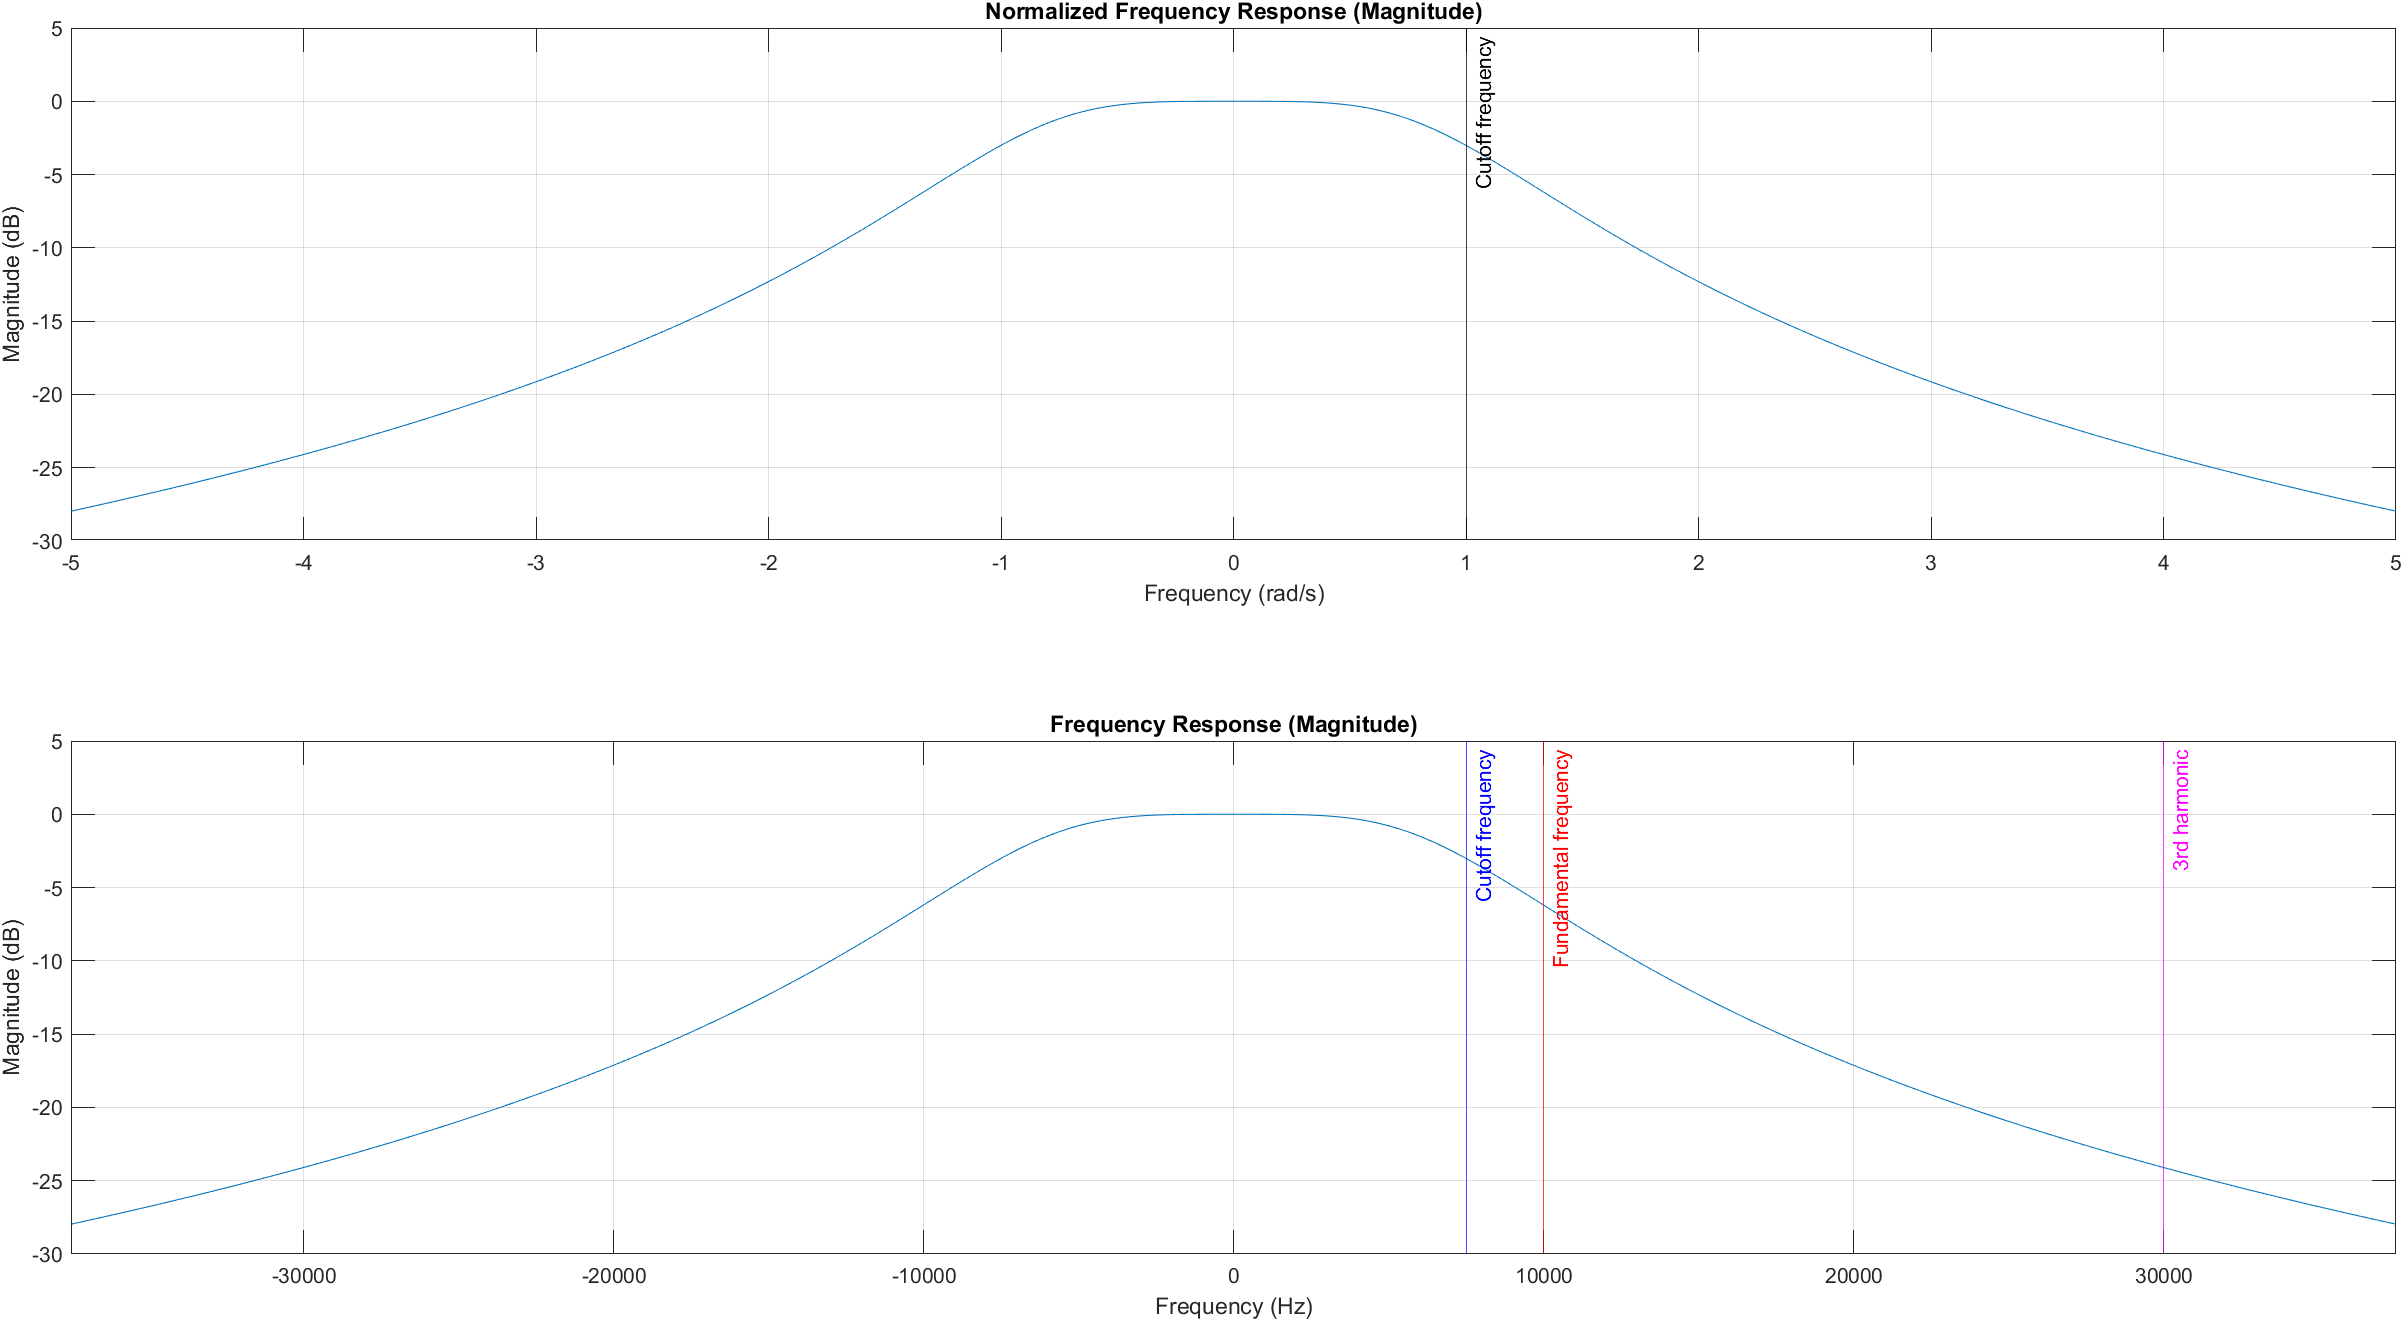
\includegraphics[width=\textwidth]{example_frequency_response.png}
    \caption{\label{fig:example_freq_response} The frequency response plots with the cutoff frequency at 7.5 kHz}
\end{figure}

\section*{Determining the Cutoff Frequency}
% determining minimum frequency to meet < 2 dB atten for fundamental attenuation 
The MATLAB script was used to determine the appropriate cutoff frequency to meet the design constraints. The first design constraint that we investigated required the loss of the fundamental sinusoid due to filtering to be less than 2 dB. We determined that this occurred when the cutoff frequency was greater than 11430 Hz. We selected a cutoff frequency of 11500 Hz, where the attenuation at the fundamental frequency was approximately 1.96 dB, as our starting point to continue and explore the other design constraints.

% figuring out what cutoff works for required attenuation from filter (23 - 9.54 = 13.46)
The other design constraint that had to be verified was the attenuation of harmonics other than at the fundamental frequency. The design problem requires any harmonics in the output to be at least 23 dB below the fundamental sinusoid. The square wave has natural attenuation that results the third harmonic being 9.54 dB below the first harmonic as calculated: $20\log_{10}\left(\frac{|C_3|}{|C_1|}\right) = 20\log_{10}\left(\frac{0.1061}{0.3183}\right) = -9.54$ dB. Therefore, the filter should provided an additional $23 - 9.54  = 13.46$ dB attenuation. When the cutoff frequency is 11.5 kHz, the attenuation provided by the filter is found to be approximately 14.79 dB, which is greater than the required 13.46 dB. Figure~\ref{fig:freq_response} shows the frequency response of the filter at 11.5 kHz. Therefore, we can conclude the minimum value of the cutoff frequency required to meet all design constraints is around 11.5 kHz.
\begin{figure}[h!]
    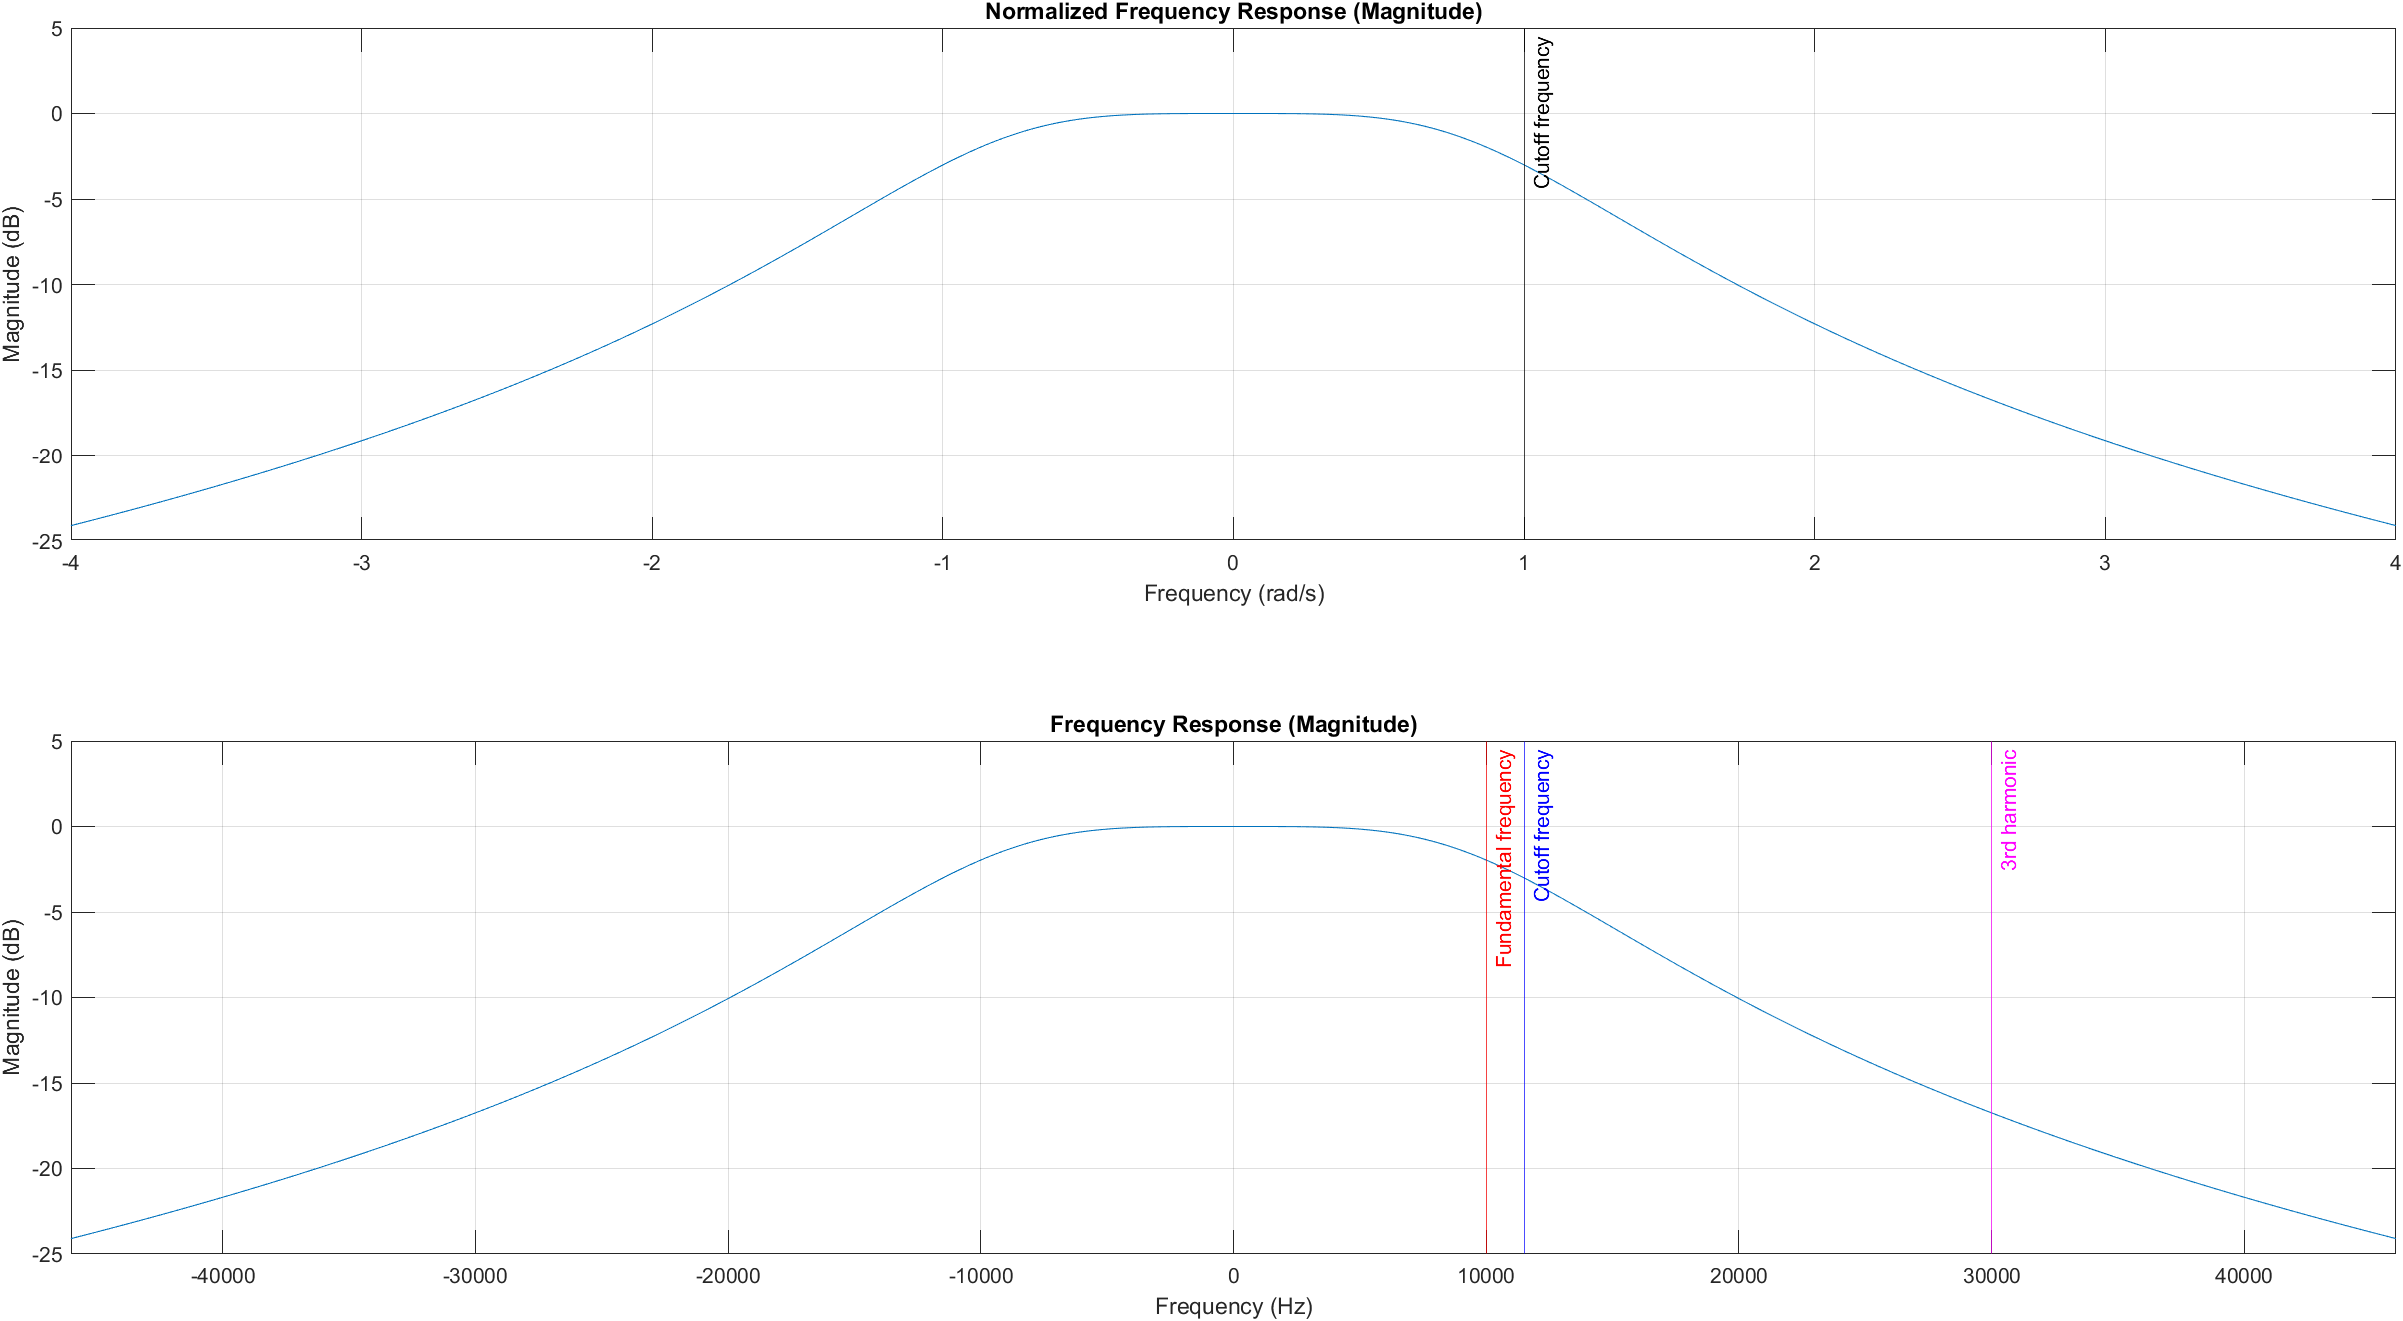
\includegraphics[width=\textwidth]{frequency_response.png}
    \caption{\label{fig:freq_response} The frequency response plots with the cutoff frequency at 11.5 kHz}
\end{figure}

\section*{Discussing the Impact of Changing Cutoff Frequency}
% Discuss the impact of changing the cutoff frequency on design constraints (For  example, what happens if the cutoff frequency is too large? Can you satisfy the  design constraint that the any harmonic in the output is at least 25 dB below the fundamental sinusoid

% range of cutoff frequencies
\section*{Determining the Range of Acceptable Cutoff Frequencies}
We have determined through simulation that the minimum cutoff frequency required to satisfy the design constraints is around 11.5 kHz. We utilize the same approach explored earlier to determine what is the maximum cutoff frequency that the filter can use while still satisfying the design constraints, and determined that the maximum cutoff frequency is around 12.9 kHz. When the cutoff frequency is set to be greater than 12.9 kHz, the filter no longer provides the required attenuation between the fundamental sinusoid and the third harmonic. Figure~\ref{fig:max_freq_response} shows the frequency response of the filter at 12.9 kHz.
\begin{figure}[h!]
    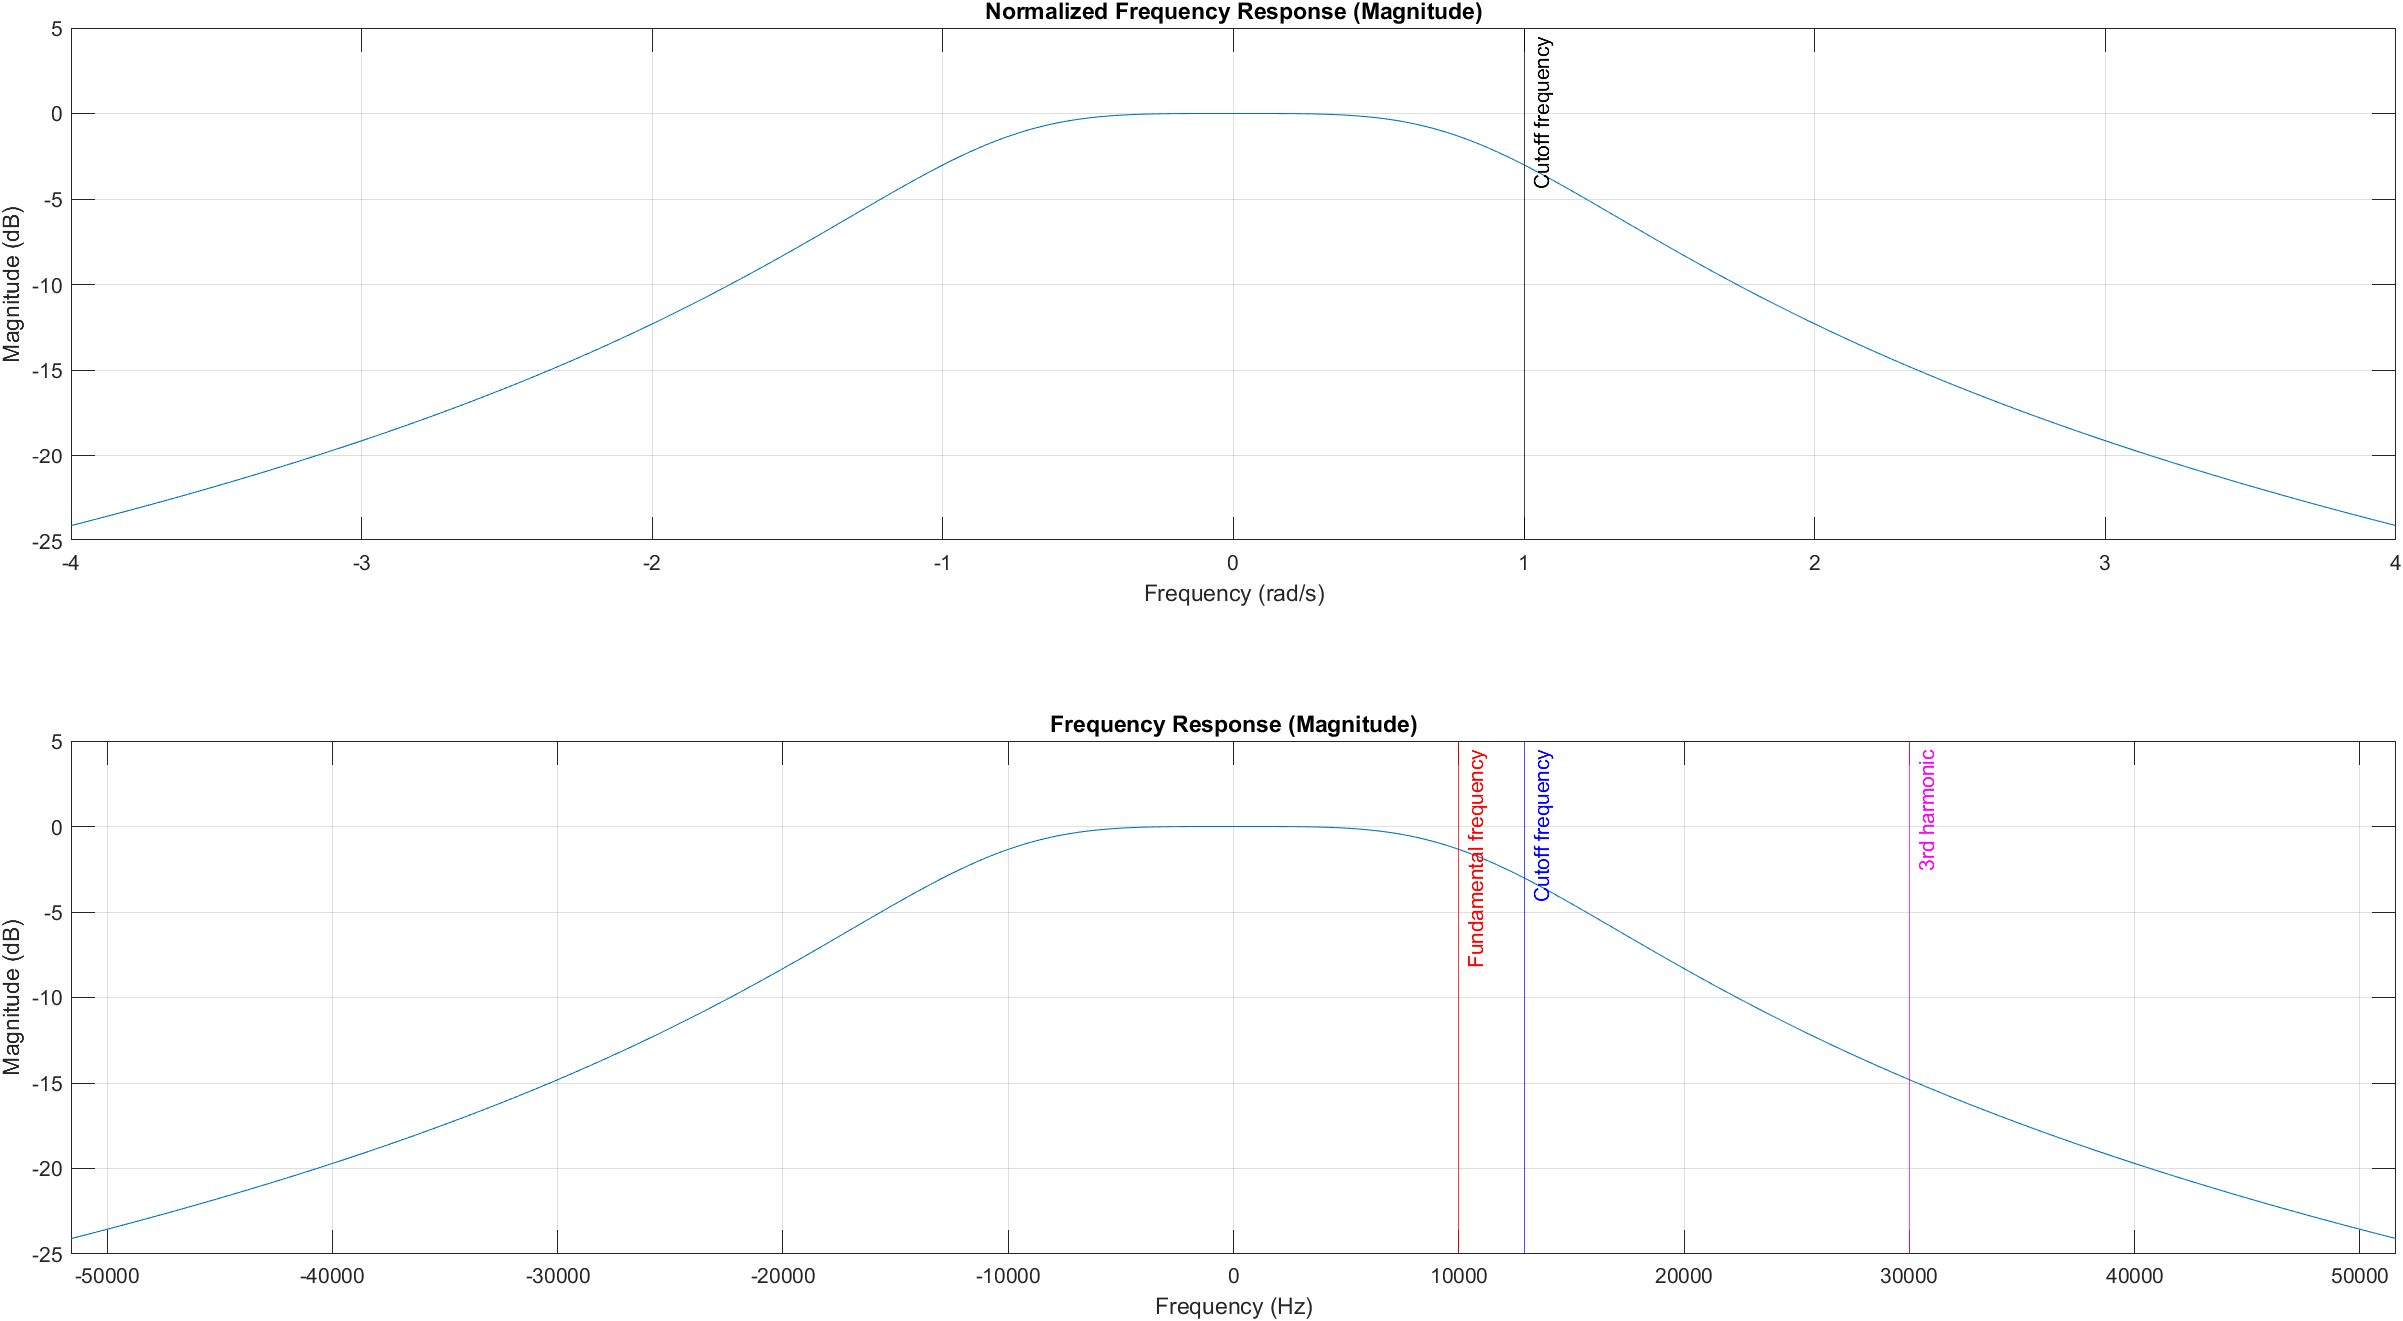
\includegraphics[width=\textwidth]{max_frequency_response.png}
    \caption{\label{fig:max_freq_response} The frequency response plots with the cutoff frequency at 12.9 kHz}
\end{figure} \\

We have determined that the acceptable range of cutoff frequencies that satisfy the design constraints of the problem are between 11.5 kHz and 12.9 kHz.

% Show analytically that the filter you have designed meets the design constraints. 
If the cutoff frequency was too large, we would not have been able to satisfy the design constraint without moving to a higher-order Butterworth filter. A larger cutoff frequency would also be detrimental to the efficacy of the filter in removing more frequency components.

% Find the range of cutoff frequencies over which the design constraints can be met (TA said we could do this either analytically or in simulation).
% If the design constraints cannot be met using the second order filter, consider using a higher order filter (TA said in tutorial u shud consider the complexity of a higher order filter if u used it).
We were able to meet the design constraints with a 2nd order filter, thus if we had to build this filter in hardware, it would be cheaper, smaller and use less resources compared a higher order filter.

% generating square wave
We used the \verb|square()| function from the Signal Processing toolbox to generate the discrete time square wave function. We generated samples from -3T_0 to +3T_0 with a step-size of 1e-7, where T_0 is 0.1ms.
% getting frequency response of square wave
% fft
% plotting magnitude spectrum
% plotting phase spectrum

% calculating output
% ifft stuff (2nd method discussed in lab)
% uh hope it actually works lol

% getting frequency response of output
In order to get the frequency response of the output signal, we took the scaled absolute value DFT of the signal, shifted it to that it was centred on the frequency (x) axis, and then plotted the resultant waveform.
\end{document}
